\chapter{The Central Limit Theorem}
\label{ch:clt}

\begin{chaptergoals}
\begin{itemize}[nosep]
\item Convergence in distribution, the mode of convergence that compares CDFs rather than values, and why its definition only looks at continuity points.
\item The Central Limit Theorem in its three equivalent forms, and what it says at the sample sizes you actually have.
\item Hoeffding's inequality: a finite-sample guarantee for bounded data when $n$ is too small to trust the CLT.
\item What the limit theorems buy you, and which of their conclusions could be reached without limits.
\end{itemize}
\Cref{ch:lln} ended with $\bar{X}_n$ collapsing onto $\mu$ and the question of what it looks like on the way there. This chapter answers it.
\end{chaptergoals}

\section{Convergence in distribution}
\label{sec:conv-dist}

Convergence in distribution is weaker than convergence in probability (and, in the full hierarchy of \cref{app:modes}, the weakest mode there is).
All it says is that the CDF of $X_n$ converges to the CDF of $X$ as $n$ goes to infinity, \textit{but doesn't require any dependence between the} $X_n$'\textit{s} \textit{and} $X$.
That is, the r.v.s $X_n$ and $X$ can be defined on entirely different probability spaces.
The CDF of these r.v.s is used instead of a PDF or PMF because all r.v.s, whether they be discrete, continuous or mixed, have CDFs.

\textbf{Question:} Why does not requiring any dependence between the $X_n$'s and $X$ make convergence in distribution weak?
You might think that, by not introducing a dependence assumption, you're actually making the statement stronger.

\textbf{Answer:} By not imposing any dependence structure between $X_n$ and $X$, convergence in distribution allows for a wider range of scenarios where the CDFs of $X_n$ converge to the CDF of $X$.
It doesn't guarantee that the actual values of $X_n$ get closer to $X$ as $n$ increases, which is a requirement for stronger forms of convergence like convergence in probability or convergence almost surely.
Convergence in distribution only concerns the limiting behavior of the distributions, not the actual values of the r.v.s.
A statement that holds in more scenarios is a weaker statement because it tells you less about any one of them.

\begin{definition}[Convergence in distribution]
\label{def:convd}
A sequence $(X_n)_{n \geq 1}$ of r.v.s \textbf{converges in distribution} to an r.v.\ $X$, denoted $X_n \convd X$, if:
\[
\lim_{n \to \infty} F_{X_n}(x) = F_X(x),
\]
for all $x$ at which $F_X$ is continuous.
\end{definition}

\begin{inwords}
\textbf{In words.} For each fixed $x$, $F_{X_n}(x) = \Pr(X_n \leq x)$ is a number, and the definition asks that this sequence of numbers converge to $\Pr(X \leq x)$, at every $x$ where the limit's CDF has no jump \toolkit{sec:math-density}. It compares two distributions, not two random variables: nothing is said about $X_n$ and $X$ being close on any outcome, and they need not even live on the same sample space.
\par\smallskip
\textbf{For the kiss data.} The CLT will say that the standardized error $\sqrt{n}(\bar{R}_n - p)/\sqrt{p(1-p)}$ converges in distribution to $\Gauss(0,1)$: for every $x$, the probability that the standardized error is below $x$ approaches $\Phi(x)$. With $n = 124$ that is the license to compute $\Pr(\abs{\bar{R}_n - p} \leq 0.084) \approx \Phi(1.95) - \Phi(-1.95) = 0.95$.
\end{inwords}

\subsection{Why only the continuity points?}

The qualifier `at which $F_X$ is continuous' looks like a technicality.
It isn't; without it the most basic examples fail.

\begin{example}
\label{ex:unif-shrinking}
Let $T_n \sim \text{Unif}\left(\left[5 - \frac{1}{2n}, 5 + \frac{1}{2n}\right]\right)$, a uniform on an interval of width $1/n$ centered at $5$.
Every sensible notion of convergence should say $T_n \to 5$, and indeed $T_n \convp 5$ since $\Pr(\abs{T_n - 5} > \delta) = 0$ as soon as $\frac{1}{2n} \leq \delta$.
The CDF $F_n$ of $T_n$ is $0$ to the left of the interval, rises linearly to $1$ across it, and in particular $F_n(5) = \frac12$ for \textit{every} $n$.
The CDF of the constant $5$ is the step function $F(t) = \ind(t \geq 5)$, with $F(5) = 1$.
So $F_n(t) \to F(t)$ for every $t \neq 5$ but not at $t = 5$, the one point where $F$ jumps.
With the continuity-point qualifier, $T_n \convd 5$; without it, $T_n$ wouldn't converge in distribution to anything.
\Cref{fig:cdfcont} shows the picture: the $F_n$ close in on the step function everywhere except at the jump, where all of them pass through $\frac12$, and the definition of convergence in distribution excludes exactly that point.
\end{example}

\begin{figure}[htbp]
\centering
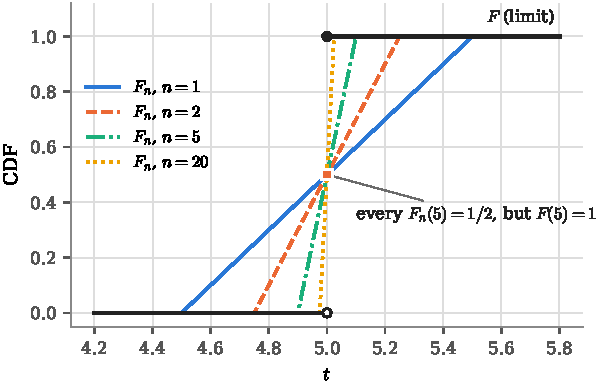
\includegraphics[width=0.7\textwidth]{fig_cdf_continuity_points}
\caption{The CDFs $F_n$ of $T_n \sim \text{Unif}([5 - \frac{1}{2n}, 5 + \frac{1}{2n}])$ for $n = 1, 2, 5, 20$, and the CDF $F$ of the constant $5$ in black. The orange square marks the point $(5, \frac12)$ that every $F_n$ passes through.}
\label{fig:cdfcont}
\end{figure}

The general principle: a jump in $F_X$ at $x$ means $X$ has positive probability of equaling $x$ exactly, and a sequence approaching from the left or the right can straddle that jump forever.
Away from the jumps there's nothing to straddle.

\subsection{Two equivalent definitions}

Alternatively, convergence in distribution can be defined using the expectation of a function, provided the function is continuous and bounded.
This is the form that generalizes: on spaces where there is no CDF to write down, it becomes the definition of convergence in distribution.

\begin{proposition}[Equivalent characterizations]
\label{prop:convd-equiv}
For real-valued r.v.s the following are equivalent:
\begin{enumerate}[nosep]
\item $F_{X_n}(x) \to F_X(x)$ for all $x$ at which $F_X$ is continuous;
\item $\E[f(X_n)] \to \E[f(X)]$ for every continuous and bounded function $f: \real \to \real$.
\end{enumerate}
If moreover $X$ has a density (for instance $X$ is Gaussian), then $X_n \convd X$ implies convergence of interval probabilities:
\[
\Pr(a \leq X_n \leq b) \to \Pr(a \leq X \leq b), \qquad \text{for all } a < b.
\]
\end{proposition}

Note that in (2) the things converging are numbers, $\E[f(X_n)]$, so the convergence is ordinary convergence of numbers.
The second form is the useful one in proofs because it doesn't single out any particular $x$; the first form is the useful one in computations because CDFs are what you can write down.
The last statement is why the CLT is enough to compute probabilities: $\Pr(a \leq Z_n \leq b) \approx \Phi(b) - \Phi(a)$, which is what every asymptotic confidence interval and test rests on.

One implication between the two modes is used on nearly every page from here on, so here it is as a statement with a proof.

\begin{proposition}[In probability implies in distribution]
\label{prop:convp-implies-convd}
If $X_n \convp X$, then $X_n \convd X$.
\end{proposition}

\optionalproof{Sandwich $F_{X_n}(x)$ between $F_X(x - \epsilon)$ and $F_X(x + \epsilon)$, up to the probability that $X_n$ and $X$ differ by more than $\epsilon$, which goes to $0$; then let $\epsilon \to 0$ and use continuity of $F_X$ at $x$. The statement is what matters; the proof is a standard $\epsilon$ argument.}
\begin{proof}
Fix a continuity point $x$ of $F_X$ and an $\epsilon > 0$.
If $X_n \leq x$ then either $X \leq x + \epsilon$ or $\abs{X_n - X} > \epsilon$, so
\[
F_{X_n}(x) \leq F_X(x + \epsilon) + \Pr(\abs{X_n - X} > \epsilon).
\]
In the same way, if $X \leq x - \epsilon$ then either $X_n \leq x$ or $\abs{X_n - X} > \epsilon$, so
\[
F_X(x - \epsilon) - \Pr(\abs{X_n - X} > \epsilon) \leq F_{X_n}(x).
\]
Let $n \to \infty$: the probability terms vanish by convergence in probability, and $F_{X_n}(x)$ is squeezed, in the limit, between $F_X(x - \epsilon)$ and $F_X(x + \epsilon)$.
Now let $\epsilon \to 0$: both bounds tend to $F_X(x)$ because $F_X$ is continuous at $x$.
\end{proof}

The continuity-point qualifier is what the last line uses: at a jump of $F_X$ the two bounds would not meet, and \cref{ex:unif-shrinking} shows the conclusion can indeed fail there.

\begin{example}
\label{ex:cos}
In \cref{ex:bern-1-over-n}, $X_n \sim \Bern(1/n)$ converges in probability, hence in distribution, to $0$.
The function $f(x) = \cos x$ is continuous and bounded, so $\E[\cos(X_n)] \to \cos(0) = 1$.
You can check this directly: $\E[\cos X_n] = (1 - \frac1n) \cos 0 + \frac1n \cos 1 \to 1$.
\end{example}

\subsection{Example 1: i.i.d.\ random variables}

If $(X_n)_{n \geq 1}$ is a sequence of i.i.d.\ r.v.s, then convergence in distribution isn't very interesting because they converge to the CDF of any one r.v.\ in the sequence.
That is, if $X_1, X_2, \ldots$ is a sequence of i.i.d.\ r.v.s with CDF $F_X(x)$, then $X_n \convd X$.
This is because:
\[
F_{X_n}(x) = F_X(x), \text{ for all } x \, \text{ implies that } \lim_{n\to \infty} F_{X_n}(x) = F_X(x), \, \text{ for all } x.
\]

This is the example from \cref{sec:conv-why}: the sequence of standard Gaussians converges in distribution to a standard Gaussian even though $\Pr(X_n = X) = 0$.
Convergence in distribution is the mode that makes sense of that example.

\subsection{Example 2: the maximum of uniforms}

\begin{example}
\label{ex:max-unif}
Let $X_1, X_2, \ldots \iid \text{Unif}([0,1])$ and define the maximum of the first $n$ by $\ds X_{(n)} = \max_{i=1,\ldots,n} X_i$.
Then:
\[
n(1 - X_{(n)}) \convd \Expo(1).
\]
\end{example}

Before the proof, a word on why the maximum is being magnified by $n$ rather than $\sqrt{n}$.
The maximum of $n$ uniforms piles up just below $1$; by the same argument as in \cref{ex:min-unif} it converges in probability to $1$, so the unmagnified sequence has a degenerate limit.
The gap $1 - X_{(n)}$ is of order $1/n$ (with $n$ points spread over $[0,1]$ the largest one sits about $1/n$ from the top), so $n$ is the magnification that holds its size fixed.
The CLT's $\sqrt{n}$ is for sums; a maximum is not a sum and gets a different rate and a different (non-Gaussian) limit.

\coreproof{Write the CDF of $n(1 - X_{(n)})$ as a probability about the whole sample, use independence to get a power $(1 - x/n)^n$, and recognize the limit $e^{-x}$ \toolkit{sec:math-explog}. Same template as \cref{ex:min-unif}, with a CDF in place of a tail probability.}
\begin{proof}
\leavevmode % Puts first item on next line
\begin{itemize}

\item Define the CDF of the r.v.\ $n(1 - X_{(n)})$ at a point $x > 0$:
\[
F_{n(1 - X_{(n)})} (x) = \Pr(n(1 - X_{(n)}) \leq x).
\]

\item Now, simplify the CDF in such a way as to eventually take the limit as $n \to \infty$.

\item To that end, observe that:
\begin{align*}
\Pr(n(1 - X_{(n)}) \leq x) &= \Pr(n - nX_{(n)} \leq x ) \\
								&= \Pr \left(X_{(n)} \geq 1 - \frac{x}{n} \right) \\
								&= 1 - \Pr \left(X_{(n)} < 1 - \frac{x}{n} \right) \\
								&= 1 - \Pr \left( X_1 < 1 - \frac{x}{n}, X_2 < 1 - \frac{x}{n}, \ldots, X_n < 1 - \frac{x}{n} \right)  \\
								&= 1 - \Pr \left(X_1 < 1 - \frac{x}{n} \right)  \Pr \left( X_2 < 1 - \frac{x}{n} \right)  \cdots \Pr \left( X_n < 1 - \frac{x}{n} \right)  \\
								&= 1 - \Pr \left( X_1 < 1 - \frac{x}{n}\right)^n.
\end{align*}

The movement from the third to the fourth equality holds because, as $X_{(n)}$ is the maximum of the $X_i$'s, the maximum is below a level exactly when every $X_i$ is below it: the single event is equivalent to the joint event.
The fifth equality results since the $X_i$'s are independent.

\item Now, recall that the $X_i$'s, and thus $X_1$, are uniformly distributed on $(0,1)$.
This means its CDF is linear, emanating from the origin rising to 1 with a slope of 1;
in other words, plug any value of the support into the CDF and you get the same value back.
Hence, for $n$ large enough that $1 - x/n \in (0,1)$:
\[
\Pr \left( X_1 < 1 - \frac{x}{n}\right) = 1 - \frac{x}{n}.
\]

\item Returning to the last right-hand side from above, you have that:
\[
1 - \Pr \left( X_1 < 1 - \frac{x}{n}\right)^n = 1 -  \left( 1 - \frac{x}{n} \right)^n,
\]

which by taking the limit as $n \to \infty$ gives:
\[
\lim_{n \to \infty} \left[ 1 -  \left( 1 - \frac{x}{n} \right)^n \right] = 1 - e^{-x},
\]

using the calculus fact $(1 - x/n)^n \to e^{-x}$.

\item To summarize, then, you have:
\[
\lim_{n \to \infty} \Pr(n(1 - X_{(n)}) \leq x) = 1 - e^{-x} \quad \text{for every } x > 0,
\]

and $1 - e^{-x}$ is the CDF of the Exponential with $\lambda = 1$ (for $x \leq 0$ both sides are $0$).
This proves the result.
\end{itemize}
\end{proof}

\Cref{fig:maxunif} shows the result by simulation.
On the left, the maximum of $n = 50$ uniforms crowds the top of the interval.
On the right, the magnified gap $n(1 - X_{(n)})$ is already very close to $\Expo(1)$ at $n = 50$.

\begin{figure}[htbp]
\centering
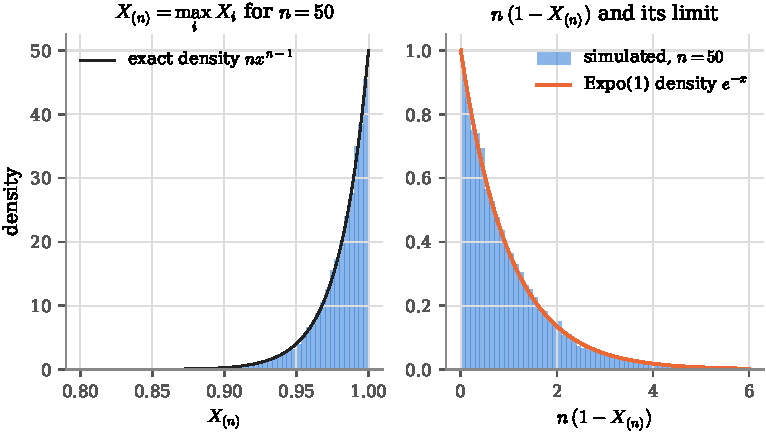
\includegraphics[width=\textwidth]{fig_max_uniform_expo}
\caption{\Cref{ex:max-unif} by simulation, $20{,}000$ replications at $n = 50$. Left: histogram of the maximum $X_{(n)}$ of $n$ uniforms, with its exact density $n x^{n-1}$ in black. Right: histogram of $n(1 - X_{(n)})$, with the $\Expo(1)$ density in orange.}
\label{fig:maxunif}
\end{figure}

\begin{pitfall}[convergence in distribution says nothing about closeness]
Let $Z \sim \Gauss(0,1)$ and set $X_n = -Z$ for every $n$.
By the symmetry of the Gaussian, $X_n \sim \Gauss(0,1)$ for every $n$, so $X_n \convd Z$.
But $\abs{X_n - Z} = 2\abs{Z}$, which is not small and never becomes small.
So $X_n$ does not converge in probability to $Z$, even though it converges in distribution to it.
Convergence in distribution is a statement about two CDFs, not about two columns of numbers getting closer.
The same example shows why you can't add limits in distribution: $X_n + Z = 0$ for every $n$, while the sum of two independent $\Gauss(0,1)$ r.v.s is $\Gauss(0,2)$.
Knowing the limiting distributions of $X_n$ and $Y_n$ separately doesn't determine the limiting distribution of $X_n + Y_n$; you need to know how they're related.
\Cref{ch:limit-tools} says what you can do instead.
\end{pitfall}


\subsection{Limits that are constants}

One case of convergence in distribution is used constantly later, so here it is as a statement with a proof.

\begin{proposition}
\label{prop:convd-constant}
If $X_n \convd c$ for a constant $c$, then $X_n \convp c$.
\end{proposition}

\optionalproof{The CDF of a constant is a step; convergence of the CDFs at two continuity points, one on each side of $c$, squeezes the mass outside the $\epsilon$-band to $0$.}
\begin{proof}
The CDF of the constant $c$ is the step $F(x) = \ind(x \geq c)$, continuous everywhere except at $c$.
Fix $\epsilon > 0$.
The points $c - \epsilon$ and $c + \epsilon/2$ are continuity points, so $F_{X_n}(c - \epsilon) \to F(c - \epsilon) = 0$ and $F_{X_n}(c + \epsilon/2) \to F(c + \epsilon/2) = 1$.
Therefore
\[
\Pr(\abs{X_n - c} \geq \epsilon) = \Pr(X_n \leq c - \epsilon) + \Pr(X_n \geq c + \epsilon) \leq F_{X_n}(c - \epsilon) + \left( 1 - F_{X_n}(c + \epsilon/2) \right) \to 0 + 0. \qedhere
\]
\end{proof}

For a constant limit, then, `in probability' and `in distribution' are the same thing, which is why the Law of Large Numbers could equally be written with the arrow for convergence in distribution, and why Slutsky's theorem in \cref{ch:limit-tools} needs only convergence in probability for the sequence with the constant limit.

\section{The Central Limit Theorem}
\label{sec:clt}

As in the previous section, let $X_1, X_2, \ldots$ be i.i.d.\ r.v.s with mean $\mu$ and variance $\sigma^2$.
The Law of Large Numbers says that as $n \to \infty$, $\bar{X}_n$ converges to the constant $\mu$.
But what is $\bar{X}_n$'s distribution along the way to becoming the constant $\mu$?
This is addressed by the Central Limit Theorem (CLT), an all-important theorem in statistics.

The CLT states that for large $n$, the distribution of $\bar{X}_n$ \textit{after standardization} approaches a standard Gaussian distribution.
Recall that if you standardize an r.v., the resulting r.v.\ is measured in units of standard deviation.
In the present case, the convergence process examines the typical deviations of $\bar{X}_n$ around $\mu$.
Now the statement of the CLT.

\begin{theorem}[Central Limit Theorem]
\label{thm:clt}
Let $\Xton$ be i.i.d.\ r.v.s such that $\E[X_i] = \mu$ and $\var(X_i) = \sigma^2 < \infty$ for $i = 1, \ldots, n$.
Then:
\[
\sqrt{n} \left( \frac{\bar{X}_n - \mu}{\sigma} \right) \convd \Gauss(0, 1).
\]
In words, the CDF of the left-hand side converges to $\Phi$, the CDF of the standard Gaussian distribution.
\end{theorem}

An equivalent statement of the CLT in which $\bar{X}_n$ remains mean-centered by $\mu$ but omits the standardization by $\sigma$ is given as follows:
\[
\sqrt{n} \left( \bar{X}_n - \mu \right) \convd \Gauss(0, \sigma^2).
\]

\textbf{Question 1:} Why does this second statement hold?

\textbf{Answer 1:} It holds because of the way the Gaussian family behaves under scaling.
Let $X \sim \Gauss(0, 1)$, so its PDF is:
\[
f_X(x) = \frac{1}{\sqrt{2 \pi} } \exp \left( - \frac{x^2}{2} \right).
\]

Now let $Y = \sigma X$ for some $\sigma > 0$.
Then $\E[Y] = \E[\sigma X] = \sigma \E[X] = 0$.
Hence the mean remains 0.
But note what happens to the variance of $X$ after multiplying it by $\sigma$:
\begin{align*}
\var(Y) = \E[(Y - \E[Y])^2] &= \E[(\sigma X - 0)^2] \\
	&= \sigma^2 \E[X^2] \\
	&= \sigma^2 \var(X) \\
	&= \sigma^2,
\end{align*}

and $Y$ is still Gaussian (a linear function of a Gaussian is Gaussian), so $\sigma X \sim \Gauss(0, \sigma^2)$.
Multiplying both sides of the first statement by the constant $\sigma$ therefore gives the second; the step `multiply both sides of a limit in distribution by a constant' is justified by the continuous mapping theorem of \cref{ch:limit-tools}.

\textbf{Question 2:} In the statement of the CLT the r.v.\ $\ds \sqrt{n} \left( \frac{\bar{X}_n - \mu}{\sigma} \right)$ converges to the standard Gaussian distribution.
The term in parentheses standardizes $\bar{X}_n$;
that is, the mean, $\mu$, is subtracted from $\bar{X}_n$, and the result divided by the standard deviation, $\sigma$.
But why multiply this standardized term by $\sqrt{n}$?

\textbf{Answer 2:} Because $\sigma$ is the standard deviation of a single $X_i$, not of $\bar{X}_n$.
The standard deviation of the sample mean equals $\sigma/\sqrt{n}$.\footnote{To see why, let $\Xton$ be i.i.d.\ r.v.s.
By independence, you have that:
\[
\var(\bar{X}_n) = \var\left( \frac{X_1}{n} + \cdots + \frac{X_n}{n} \right) = \frac{\sigma^2}{n^2} + \cdots + \frac{\sigma^2}{n^2} = \frac{n \sigma^2}{n^2} = \frac{\sigma^2}{n}.
\]}
Standardizing $\bar{X}_n$ properly means dividing by \textit{its} standard deviation, and division by a fraction is multiplication by its reciprocal:
\[
\frac{\bar{X}_n - \mu}{\sigma/\sqrt{n}} = \sqrt{n} \left( \frac{\bar{X}_n - \mu}{\sigma} \right).
\]
So the $\sqrt{n}$ isn't an extra factor; it's the part of the standardization that's easy to lose track of.

A third and equivalent statement of the CLT uses a standardized sum.
Define the standardized sum of $X_1 + \cdots + X_n$ by:
\[
Z_n = \frac{n \bar{X}_n - n \mu}{\sqrt{n} \sigma},
\]

where $n \bar{X}_n$ is just $X_1 + \cdots + X_n$.
As $Z_n$ is standardized it follows that $\E(Z_n) = 0$ and $\var(Z_n) = 1$.
Further, let $Z$ be a standard Gaussian r.v.
Then the CLT states that:
\[
\lim_{n \to \infty} \Pr(Z_n \leq z) = \Pr(Z \leq z), \text{ for every } z,
\]

where $\Pr(Z \leq z)$ is the standard Gaussian CDF $\Phi(z)$.
The reason why the CLT states that the CDF of $Z_n$ (and not its PDF) converges to the standard Gaussian CDF is because the result applies to \textit{all} r.v.s with finite variance, and all r.v.s have CDFs.
The $X_i$ can be discrete, as in the kiss experiment, in which case $Z_n$ has no PDF at all.

\textbf{Question 3:} Why do you standardize the sums of the $X_i$'s for the approximation?

\textbf{Answer 3:} Suppose the $X_1 + \cdots + X_n$ aren't standardized.
Then $\E(X_1 + \cdots + X_n) = n \mu$ and $\var(X_1 + \cdots + X_n) = n \sigma^2$.
Both are finite for every $n$, but neither stays bounded as $n \to \infty$: the unstandardized sum drifts off (its mean is $n\mu$) and spreads out (its standard deviation is $\sigma\sqrt{n}$), so no fixed distribution can describe it and its CDF has no limit that is a CDF.
Standardizing pins the sum down, with $\E(Z_n) = 0$ and $\var(Z_n) = 1$ for all $n$, so that a limiting distribution has a chance to exist.

\begin{figure}[htbp]
\centering
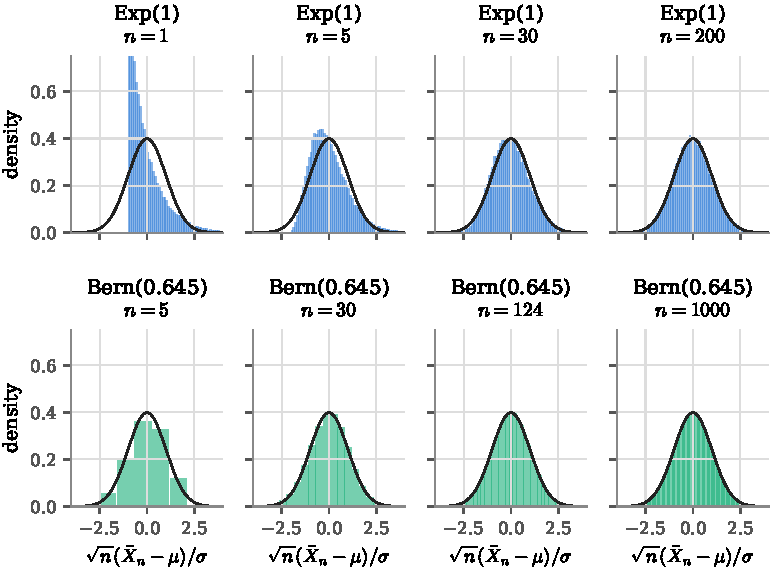
\includegraphics[width=\textwidth]{fig_clt_in_action}
\caption{The standardized sample mean $\sqrt{n}(\bar{X}_n - \mu)/\sigma$, with the $\Gauss(0,1)$ density in black over it. Top row: $\Expo(1)$ draws at $n = 1, 5, 30, 200$, histograms from $50{,}000$ simulated samples. Bottom row: $\Bern(0.645)$ draws at $n = 5, 30, 124, 1000$, the exact Binomial distribution as bars.}
\label{fig:cltaction}
\end{figure}

\begin{bridge}[the `$n \geq 30$' rule]
Introductory courses offer a rule of thumb: the normal approximation to the sample mean is fine once $n \geq 30$.
The CLT contains no such number.
It's a limit statement, and how fast the limit is reached depends on the parent distribution: above all on how asymmetric and heavy-tailed it is.
In the top row of \cref{fig:cltaction} the parent is the strongly skewed $\Expo(1)$, and the skew is still visible at $n = 30$.
In the bottom row the parent is the kiss experiment's $\Bern(0.645)$; the standardized mean lives on a lattice, visible as bars, and by $n = 124$ the Gaussian is already an excellent description.
For a symmetric parent, $n = 5$ can be enough; for a heavily skewed one, $n = 200$ may not be.
What is a theorem is the \textit{rate}: the Berry--Esseen bound says the gap between the CDF of $Z_n$ and $\Phi$ is at most a universal constant times $\E\abs{X - \mu}^3 / (\sigma^3 \sqrt{n})$, so the error shrinks like $1/\sqrt{n}$, slowly when the ratio $\E\abs{X - \mu}^3/\sigma^3$ is large, as it is for skewed and heavy-tailed parents.
A finer expansion (the Edgeworth expansion) shows that, for a continuous parent, the leading term of the error is proportional to the parent's skewness, which is why symmetric parents reach the Gaussian faster in practice.
\end{bridge}

\subsection{The essence of the CLT: a `stochastic' bound}

Due to the so-called `empirical rule', values between $-3$ and $3$ in the support of a standard Gaussian account for nearly 100\% of its probability mass ($99.7\%$ of it).
By the CLT, this implies that, for $n$ large enough for the approximation to apply, the following inequality holds with probability about $99.7\%$:
\[
\abs{\bar{X}_n - \mu} \leq \frac{3 \sigma}{\sqrt{n}},
\]

since, for every $n$, the two events are the same:
\begin{align*}
\sqrt{n} \left( \frac{\bar{X}_n - \mu}{\sigma} \right) \in [-3, 3] &\Leftrightarrow -3 \leq \sqrt{n} \left( \frac{\bar{X}_n - \mu}{\sigma} \right) \leq 3 \\
&\Leftrightarrow \abs*{ \sqrt{n} \left( \frac{\bar{X}_n - \mu}{\sigma} \right) } \leq 3 \\
&\Leftrightarrow \frac{\sqrt{n}}{\sigma} \abs{ \bar{X}_n - \mu } \leq 3 \\
&\Leftrightarrow \abs{ \bar{X}_n - \mu } \leq  \frac{3 \sigma}{\sqrt{n}}.
\end{align*}

The essence of the CLT is that, despite $\bar{X}_n - \mu$ being an r.v.\ with an unbounded support (when the $X_i$ are unbounded), it's \textit{stochastically} bounded in the sense that, with high probability, it's between $-3\sigma/\sqrt{n}$ and $3\sigma/\sqrt{n}$.
Replace $3$ by $1.96$ and `with high probability' by $95\%$ and you have the recipe for every confidence interval in \cref{ch:confidence-intervals}.
\Cref{fig:funnel} draws the bound as a funnel around the running average, and it is also the chapter's two theorems in one picture.
The funnel narrows like $1/\sqrt{n}$: that is the Law of Large Numbers.
At any fixed $n$ past the first few dozen, about $5\%$ of the paths are outside the inner funnel and almost none outside the outer one (in this simulation, $6\%$ of the points with $n \geq 30$ are outside the inner funnel): that is the stochastic bound.
The inner funnel at $n = 124$ is the width of the confidence interval of \cref{ch:confidence-intervals}.

\begin{bridge}[the `$np \geq 10$ and $n(1 - p) \geq 10$' condition]
An introductory course says the sample proportion is approximately normal, with mean $p$ and standard deviation $\sqrt{p(1-p)/n}$, once $np \geq 10$ and $n(1 - p) \geq 10$ (some books say $5$, some $15$).
That is \cref{thm:clt} for $\Bern(p)$ data, with $\mu = p$ and $\sigma^2 = p(1-p)$; the inner funnel of \cref{fig:funnel} is $p$ plus or minus $1.96$ of those standard deviations.
The condition is stated in counts rather than in $n$ because the Bernoulli parent's skewness, $(1 - 2p)/\sqrt{p(1-p)}$, grows without bound as $p$ nears $0$ or $1$, and the skewness of the count is that divided by $\sqrt{n}$.
With both counts at least $10$ the count's skewness is at most $1/\sqrt{10} = 0.32$ in size, whatever $p$ is; at $p = 0.01$ the condition asks for $n = 1{,}000$, where the `$n \geq 30$' rule would accept $n = 30$ and a skewness of $1.8$.
For the kiss data the counts, with $\hat{p}$ in place of $p$, are the observed $80$ and $44$, and the count's skewness is $-0.05$.
\Cref{sec:tests-kiss} takes up the continuity correction, which repairs the count's discreteness rather than its skewness.
\end{bridge}

\begin{figure}[htbp]
\centering
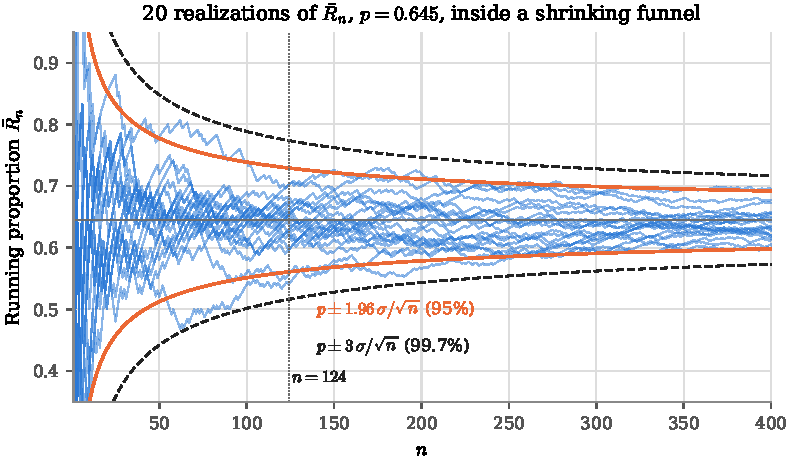
\includegraphics[width=\textwidth]{fig_clt_funnel}
\caption{Twenty realizations of the running proportion $\bar{R}_n$ in the kiss model, $p = 0.645$, with the curves $p \pm 1.96\,\sigma/\sqrt{n}$ (orange) and $p \pm 3\,\sigma/\sqrt{n}$ (dashed black), where $\sigma = \sqrt{p(1-p)}$. The dotted line marks $n = 124$.}
\label{fig:funnel}
\end{figure}

\section{Hoeffding's inequality: help for small sample sizes}
\label{sec:hoeffding}

What if your sample size, $n$, is not large enough to apply the CLT?
Hoeffding's inequality is a helpful tool when $n$ is small that effectively delivers the same essential message as the CLT: $\bar{X}_n$ is close to $\mu$ within some stochastic bound.
The statement isn't as strong as the CLT and requires additional restrictions on the r.v.s.
Namely, the r.v.s must be bounded almost surely, that is, with probability one \toolkit{sec:math-rv}, which rules out any r.v.\ with an arbitrarily large or small support (e.g., Gaussian and Exponential r.v.s).
But despite the stronger restrictions, its power lies in providing a bound on the distance between $\bar{X}_n$ and $\mu$ that is a theorem rather than an approximation, for every $n$, however small.
Here's the statement.

\begin{theorem}[Hoeffding's inequality, 1963]
\label{thm:hoeffding}
Let $n$ be some positive integer and $X, \Xton$ be i.i.d.\ r.v.s such that $\mu = \E[X]$ and $X$ is almost surely bounded within $[a,b]$ where $a < b$.
Then:
\[
\Pr\left( \abs{ \bar{X}_n - \mu } \geq \epsilon \right) \leq 2 \exp \left( - \frac{2n\epsilon^2}{(b-a)^2} \right), \, \, \text{ for all } \epsilon > 0.
\]
\end{theorem}

Compare this with Chebyshev's bound $\sigma^2/(n \epsilon^2)$.
Both go to zero as $n$ grows, but Hoeffding's bound goes to zero \textit{exponentially} fast in $n$ while Chebyshev's goes like $1/n$.
The price is the boundedness assumption, which Chebyshev doesn't need.
Note also what Hoeffding's inequality is not: it's a bound, not an approximation.
The CLT says $\Pr(\abs{\bar{X}_n - \mu} \geq \epsilon) \approx 2(1 - \Phi(\epsilon \sqrt{n}/\sigma))$ for large $n$ without saying how large; Hoeffding says $\Pr(\abs{\bar{X}_n - \mu} \geq \epsilon) \leq 2e^{-2n\epsilon^2/(b-a)^2}$ for every $n \geq 1$, full stop.

\begin{worked}[the kiss experiment, three ways]
The $R_i$ are Bernoulli, so they're bounded in $[0, 1]$ and $(b - a)^2 = 1$.
With $n = 124$ and $\epsilon = 0.084$:
\begin{itemize}[nosep]
\item Chebyshev (with $p(1-p)$ evaluated at $0.645$): $\Pr(\abs{\bar{R}_n - p} \geq 0.084) \leq 0.26$; with the worst case $p(1-p) \leq 1/4$ instead, $0.29$.
\item Hoeffding: $\Pr(\abs{\bar{R}_n - p} \geq 0.084) \leq 2 \exp(-2 \times 124 \times 0.084^2) = 2 e^{-1.75} \approx 0.35$.
\item CLT: $\Pr(\abs{\bar{R}_n - p} \geq 0.084) \approx 2 \left( 1 - \Phi \left( \frac{0.084 \sqrt{124}}{\sqrt{0.645 \times 0.355}} \right) \right) = 2(1 - \Phi(1.95)) \approx 0.05$.
\end{itemize}
At this $n$ the exact Binomial probability is $0.05$, so the CLT approximation is right on and both bounds are loose, with Chebyshev slightly tighter than Hoeffding.
\Cref{fig:bounds} shows that Hoeffding overtakes Chebyshev at about $n = 165$ and is far ahead by $n = 400$, as the exponential must eventually beat $1/n$.
In the figure the CLT approximation sits on top of the exact probability for $n$ beyond a few dozen.
The jaggedness of the exact curve is real: it comes from the lattice of possible values of $\bar{R}_n$ moving relative to the fixed $\epsilon$.
The two bounds are guarantees; the CLT number is an approximation that happens, here, to be excellent.
\end{worked}

\begin{figure}[htbp]
\centering
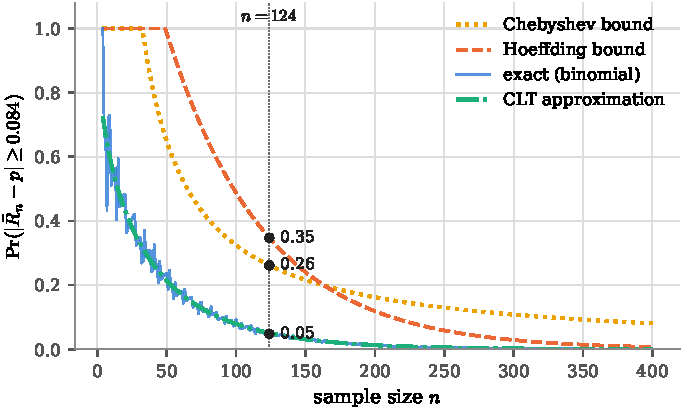
\includegraphics[width=0.85\textwidth]{fig_bounds_vs_truth}
\caption{$\Pr(\abs{\bar{R}_n - p} \geq 0.084)$ in the kiss model with $p = 0.645$, as a function of $n$: the exact Binomial probability, the CLT approximation, and the Chebyshev and Hoeffding upper bounds. The dots mark $n = 124$.}
\label{fig:bounds}
\end{figure}

\section{What the limit theorems buy you}
\label{sec:conv-what-limits-buy}

A fair question at this point: couldn't the results of this chapter and the last be proved without limits?
More of them than you would guess, and it's worth seeing which because it shows what the limit theorems are actually for.

\textbf{Results that have a finite-sample version.}
\begin{itemize}
\item The Law of Large Numbers is Chebyshev's inequality with $n$ sent to infinity.
The finite-$n$ content is the inequality itself, $\Pr(\abs{\bar{X}_n - \mu} \geq \epsilon) \leq \sigma^2/(n\epsilon^2)$; the limit only tidies the statement.
Hoeffding's inequality (\cref{sec:hoeffding}) is the same idea with a better bound; the `conservative' confidence interval of \cref{ch:confidence-intervals} uses the same trick of replacing the unknown variance by its worst case, $p(1-p) \leq 1/4$.
Both are guarantees that hold at $n = 2$ as well as at $n = 10^6$.
\item When the parent distribution is known, an exact sampling distribution replaces the CLT.
For Bernoulli data the sum $n\bar{R}_n$ is Binomial, so the kiss experiment's proportion has exact tests and an exact interval (the Clopper--Pearson interval, which for these data is $[0.55, 0.73]$).
For Exponential data the sum is Gamma, which gives an exact interval for the subway rate $\lambda$ (an exercise in \cref{ch:confidence-intervals}).
For Gaussian data the standardized mean has a $t$ distribution and the ratio of variances an $F$ distribution, which is why the $t$-test of \cref{ch:t-test} and Gaussian linear regression in \cref{ch:regression-multi} need no limit theorem at all.
\item The CLT itself has a finite-sample version: the Berry--Esseen theorem mentioned in \cref{sec:clt} bounds the gap between the CDF of the standardized mean and $\Phi$ at every $n$.
The limit statement is that theorem with the error term dropped.
\end{itemize}

\textbf{What has no finite-sample substitute.}
What you can't do without a limit theorem is get a statement that is both universal and sharp.
Chebyshev and Hoeffding hold for every parent too, but as bounds that may sit far from the truth; an approximation that is accurate for every parent at once is the whole content of the CLT.
It's the only reason the same recipe, estimate $\pm 1.96 \times$ standard error, works for proportions, means, rates, regression coefficients and maximum likelihood estimators of every model in this book.
Without it you must either know the parent exactly, and then compute its exact sampling distribution, which is possible for the three families above and intractable for most others, or accept an inequality, which is honest but often far from the truth: Hoeffding says $0.35$ where the exact answer is $0.05$ in the kiss experiment (\cref{fig:bounds}).
The asymptotic normality of a general maximum likelihood estimator (\cref{ch:mle-properties}) and Wilks' theorem for the likelihood ratio test (\cref{ch:wald-lrt}) have no finite-sample versions; their exact distributions depend on the model and are usually unobtainable.

So the asymptotic route is a trade: one formula for every model, in exchange for not knowing how large $n$ must be.
The price is paid in the places where the approximation is poor, which the Berry--Esseen bound says are the heavy-tailed and asymmetric parents, and small $n$.

\section{What comes next}
\label{sec:clt-next}

You now have two limits for the sample mean: it collapses onto $\mu$ (\cref{ch:lln}) and, magnified by $\sqrt{n}$, its error is Gaussian (this chapter).
Almost nothing in statistics is literally a sample mean.
The estimator of the subway rate is $1/\bar{T}_n$, the standard error you can compute has $\hat{p}$ where the CLT has $p$, and the odds are a ratio of two things.
The next chapter is the toolkit for carrying the two limits through such operations: Slutsky's theorem for plugging in, the continuous mapping theorem for transforming, and the delta method for the CLT of a function of an average.

\section{Summary}
\label{sec:clt-summary}

\begin{itemize}[nosep]
\item \textbf{Convergence in distribution:} $X_n \convd X$ if $F_{X_n}(x) \to F_X(x)$ at every continuity point of $F_X$; equivalently $\E[f(X_n)] \to \E[f(X)]$ for every bounded continuous $f$. It compares distributions, not values: $X_n = -Z$ converges in distribution to $Z$ without ever being close to it.
\item Convergence in probability implies convergence in distribution (\cref{prop:convp-implies-convd}). The converse can fail, as the $X_n = -Z$ example shows, unless the limit is a constant, in which case it holds (\cref{prop:convd-constant}).
\item \textbf{Central Limit Theorem:} $\sqrt{n}(\bar{X}_n - \mu)/\sigma \convd \Gauss(0,1)$, whatever the parent distribution with finite variance. With overwhelming probability $\abs{\bar{X}_n - \mu} \leq 3\sigma/\sqrt{n}$: a funnel that narrows like $1/\sqrt{n}$. How fast the Gaussian arrives depends on the parent, above all on its asymmetry; the `$n \geq 30$' rule is a convention.
\item Averages are not the only things with limits, and $\sqrt{n}$ and the Gaussian are not the only rate and limit: the maximum of $n$ uniforms has an error of order $1/n$ and an Exponential limit (\cref{ex:max-unif}).
\item \textbf{Hoeffding's inequality:} for data in $[a,b]$, $\Pr(\abs{\bar{X}_n - \mu} \geq \epsilon) \leq 2 e^{-2n\epsilon^2/(b-a)^2}$ for every $n$. A guarantee, not an approximation, and exponentially better than Chebyshev for large $n$.
\item The limit theorems' content is universality: one formula for every parent. The price is not knowing how large $n$ must be. When the parent is known, exact distributions (Binomial, Gamma, $t$, $F$) need no limits at all.
\end{itemize}

\section{Exercises}
\label{sec:clt-exercises}

\begin{exercise}
Let $T_n \sim \text{Unif}([5 - \frac{1}{2n}, 5 + \frac{1}{2n}])$. (a) For a fixed $0 < \delta < 1$, find $N$ such that $\Pr(\abs{T_n - 5} > \delta) = 0$ whenever $n \geq N$. (b) What is the limit of $(T_n)$? (c) Let $F_n$ be the CDF of $T_n$ and $F$ the CDF of the limit. For which $t$ does $F_n(t) \to F(t)$?
\end{exercise}
\begin{solution}
(a) $\abs{T_n - 5} \leq \frac{1}{2n}$ always, so the probability is $0$ as soon as $\frac{1}{2n} \leq \delta$, i.e., for $n \geq \frac{1}{2\delta}$; any $N \geq \frac{1}{2\delta}$ works. (b) $T_n \convp 5$ (and so also in distribution). (c) For all $t \neq 5$: $F_n(5) = \frac12$ for every $n$ while $F(5) = 1$. See \cref{ex:unif-shrinking} and \cref{fig:cdfcont}.
\end{solution}

\begin{exercise}
Let $Y_1, Y_2, \ldots \iid \text{Unif}([0,1])$ and $M_n = \max(Y_1, \ldots, Y_n)$. (a) For $0 < \delta < 1$, find $\Pr(\abs{M_n - 1} > \delta)$. (b) Does $M_n$ converge in probability to a constant? (c) Find the CDF of $M_n$ on $[0,1]$.
\end{exercise}
\begin{solution}
(a) Since $M_n \leq 1$, $\Pr(\abs{M_n - 1} > \delta) = \Pr(M_n < 1 - \delta) = \Pr(Y_1 < 1 - \delta)^n = (1 - \delta)^n$. (b) Yes: $(1-\delta)^n \to 0$, so $M_n \convp 1$. (c) $F_{M_n}(x) = \Pr(Y_1 \leq x, \ldots, Y_n \leq x) = x^n$. As $n \to \infty$ this tends to $0$ for $x < 1$ and equals $1$ at $x = 1$: the CDF of the constant $1$, at its continuity points.
\end{solution}

\begin{exercise}
Let $\Xton \iid \text{Unif}([0, b])$, so $\sigma^2 = b^2/12$, with $n$ too small to trust the CLT. Find the Chebyshev and Hoeffding upper bounds on $\Pr(\abs{\bar{X}_n - \E[X]} \geq c\,\sigma/\sqrt{n})$ for $c = 2$ and $c = 6$.
\end{exercise}
\begin{solution}
Chebyshev with $\epsilon = c\sigma/\sqrt{n}$ gives $\frac{\sigma^2/n}{c^2 \sigma^2/n} = 1/c^2$: $0.25$ for $c = 2$ and $0.028$ for $c = 6$. Hoeffding with $(b - a)^2 = b^2$ gives $2\exp(-2n\epsilon^2/b^2) = 2\exp(-2c^2\sigma^2/b^2) = 2 e^{-c^2/6}$: $2e^{-2/3} = 1.03$ (useless, since a probability is at most $1$) for $c = 2$, and $2e^{-6} = 0.005$ for $c = 6$. Chebyshev wins for small $c$; Hoeffding's bound decays like $e^{-c^2/6}$ against Chebyshev's $1/c^2$, so Hoeffding wins once $c$ is large, exactly as in \cref{fig:bounds} with $n$ in place of $c$.
\end{solution}

\begin{exercise}
In the kiss experiment, use the CLT to find the smallest $n$ for which $\Pr(\abs{\bar{R}_n - p} \geq 0.02) \approx 0.05$ when $p = 0.645$, and compare with the Chebyshev answer of \cref{sec:lln-exercises}.
\end{exercise}
\begin{solution}
The CLT gives $\Pr(\abs{\bar{R}_n - p} \geq \epsilon) \approx 2(1 - \Phi(\epsilon\sqrt{n}/\sqrt{p(1-p)}))$, which equals $0.05$ when $\epsilon \sqrt{n}/\sqrt{p(1-p)} = 1.96$, i.e., $n = 1.96^2 \times 0.229/0.02^2 \approx 2{,}200$. Chebyshev demanded about $11{,}450$, five times as many, for the same guarantee.
\end{solution}
